\documentclass[12pt]{article}
\usepackage{polyglossia}
\setdefaultlanguage{french}
\usepackage{fontspec}
\usepackage{graphicx}
\usepackage{amssymb}
\usepackage{hyperref}
\emergencystretch=2.5em

\title{IFT3295 - TP2}
\author{Repliement d'ARN et alignement multiple}
\date{9 octobre 2026}

\begin{document}

\maketitle
\section*{Évaluation}
\begin{itemize}
	\item Ce TP est à faire en équipe de deux (pas d'équipe de trois).
	\item Vous devez le rendre au plus tard le
	      mercredi 28 octobre 2026 avant la démo (avant 13~h~29).
	\item Deux fichiers à remettre : un zip du squelette complété et un pdf
	      pour les autres questions.
	\item Utiliser Studium pour la remise du TP. Une version papier des réponses écrites est aussi
	      acceptée.
	\item \textbf{Vous devez utiliser le squelette de code fourni avec le TP}
	      (\texttt{main.py}, \texttt{alignement.py}, \texttt{etoile.py}, \texttt{utils.py},
	      \texttt{run.sh}) : complétez les fonctions marquées
	      \texttt{NotImplementedError \# TODO}. Vous pouvez ajouter des imports
	      de la bibliothèque standard et définir des fonctions auxiliaires dans
	      \texttt{alignement.py} et \texttt{etoile.py}, en annotant leurs paramètres
	      et leurs retours. Ne modifiez pas les noms, signatures ou annotations
	      des fonctions fournies, ni les constantes. Ne modifiez pas
	      \texttt{main.py}, \texttt{utils.py} ou \texttt{run.sh}.
	      Le script \texttt{run.sh} exécute le
	      pipeline complet (matrice de similarité, alignement étoile, score SP,
	      consensus, copie modifiée de la séquence centrale et réalignement).
	\item \textbf{Il est formellement interdit d'utiliser des bibliothèques
	      externes pour l'alignement de séquences} :
	      vous devez implémenter vous-même les algorithmes, avec la bibliothèque
	      standard de Python seulement.
	\item Votre code doit être bien lisible et compréhensible (bonne
	      indentation, noms de variables et de fonctions représentatifs, commentaires,
	      etc.).
\end{itemize}

\subsection*{Exécution du squelette}

Utilisez \textbf{Python 3.10 ou ultérieur}, sans dépendance externe à installer.
Depuis le dossier du squelette, lancez le pipeline complet avec :
\begin{verbatim}
bash run.sh
\end{verbatim}
Le script produit dans ce dossier :
\begin{itemize}
	\item \texttt{similarite.csv} : la matrice de similarité (Q1) ;
	\item \texttt{alignement.fasta} : l'alignement étoile (Q3) ;
	\item \texttt{realignement.fasta} : le nouvel alignement (Q7).
\end{itemize}
Tant que les fonctions nécessaires ne sont pas complétées, une erreur
\texttt{NotImplementedError} est normale ; le script s'arrête à la première erreur.

Pour exécuter uniquement la question 1 :
\begin{verbatim}
python3 main.py paires sequences.fasta BLOSUM62.txt
\end{verbatim}
Pour exécuter les questions 2 à 7 (la question 1 doit aussi être implémentée) :
\begin{verbatim}
python3 main.py etoile sequences.fasta BLOSUM62.txt
\end{verbatim}
Pour calculer le score SP d'un alignement au format FASTA ou Clustal :
\begin{verbatim}
python3 main.py sp <fichier> BLOSUM62.txt
\end{verbatim}
Remplacez \texttt{<fichier>} par le chemin de l'alignement à évaluer.

\section*{Repliement d'ARN en tige-boucle (45 pts)}

La prédiction de la structure secondaire des ARN est un problème classique de la biologie computationnelle : la forme qu'adopte un ARN conditionne son rôle dans la cellule et guide notamment la recherche de nouvelles molécules thérapeutiques. Ce problème se résout élégamment par programmation dynamique.

Pour les questions 1 à 6, étant donné une séquence d'ARN $S$, on veut retrouver le repliement en une tige-boucle (figure~\ref{fig:tige}) de $S$ qui maximise le nombre d'appariements de bases.

\begin{figure}[htbp]
	\centering
	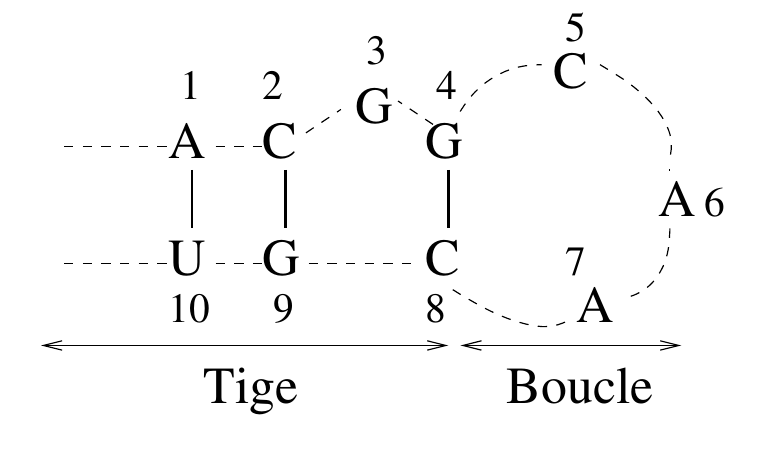
\includegraphics[scale=0.4]{tigeboucle.png}
	\caption{Tige-boucle}
	\label{fig:tige}
\end{figure}

Notez qu'une tige-boucle peut contenir des nucléotides non appariés et que seuls les appariements (A-U et G-C) sont considérés.

Ce problème peut être ramené à celui de l'identification du plus grand nombre de «~match~» entre une sous-séquence de $S$ et une autre de la séquence inverse et complémentaire $S_r$ de $S$. Il s'agit de la séquence obtenue en lisant $S$ de droite à gauche et en remplaçant chaque nucléotide par le nucléotide complémentaire (A par U, C par G, et inversement).
Par exemple, si $S$ est la séquence de la figure~\ref{fig:tige} ($S = \mathrm{ACGGCAACGU}$), alors $S_r = \mathrm{ACGUUGCCGU}$.

Décrivez un algorithme de programmation dynamique (fonctionnant en temps $O(n^2)$ pour une séquence de longueur $n$) qui remplit une table $M$ (indicée à 0, où les lignes et colonnes d'indice 0 représentent des chaînes vides) et permet de retrouver un repliement en tige-boucle maximisant le nombre d'appariements, en identifiant le plus grand nombre de «~match~» entre une sous-séquence de $S$ et une autre de $S_r$. Pour ce faire :
\begin{enumerate}
	\item À quoi correspondent les cellules de $M$ sur l'anti-diagonale ($M[i, |S|-i]$) ? Faut-il remplir toute la table ? (5 pts)
	\item Donnez les équations d'initialisation et de récurrence pour remplir la table $M$. (10 pts)
	\item Décrivez comment retrouver un repliement en tige-boucle maximisant les appariements de nucléotides. (5 pts)
	\item Appliquez votre algorithme à $\mathrm{GCGUGCUUGCGUGCACG}$. On vous demande la table de programmation dynamique, le score, ainsi que le repliement. Donnez la liste des paires appariées $(i, j)$ et un dessin en notation points-parenthèses. (15 pts)
	\item Pour être stable, la boucle de la tige-boucle doit contenir au moins 3 nucléotides. Décrivez une façon de modifier votre algorithme afin d'avoir des tige-boucles avec au moins 3 nucléotides dans la boucle. (5 pts)
	\item Décrivez une modification de votre algorithme qui permet les appariements G-U. (5 pts)
\end{enumerate}

\section*{Alignement multiple de séquences (55 pts)}

Aligner plusieurs séquences simultanément permet de repérer les régions conservées au sein d'une famille de gènes : c'est la base de l'analyse phylogénétique, de la détection d'homologie et de l'annotation fonctionnelle des gènes. Le calcul exact étant hors de portée dès qu'on dépasse deux séquences, on a recours à des heuristiques, dont la méthode de l'étoile.

\subsection*{Alignement avec arbre étoile (45 pts)}

Soit $\mathbb{S} = \{S_1, S_2, S_3, S_4, S_5\}$ un ensemble de séquences protéiques appartenant à la même famille de gènes (fichier \texttt{sequences.fasta} du squelette).

On vous demande un alignement multiple de ces séquences par la méthode de l'étoile centrale. Le fichier \texttt{BLOSUM62.txt} contient le score entre chaque paire d'acides aminés. Le symbole «~\texttt{*}~» de cette matrice désigne un codon stop, pas un gap : les gaps, notés «~\texttt{-}~», ne sont jamais lus dans BLOSUM62. La pénalité affine d'un run de $k$ gaps est $-(a + kb)$, avec $a = 10$ et $b = 1$. Les gaps aux extrémités sont pénalisés (alignement global).

Les questions 1 à 7 sont calculées par le programme du squelette (Q1 : \texttt{alignement\_global} et \texttt{matrice\_similarite} ; Q2 : \texttt{sequence\_centrale} ; Q3 : \texttt{alignement\_etoile} ; Q4 : \texttt{score\_sp} ; Q5 : \texttt{sequence\_consensus} ; Q6 : \texttt{sequence\_modifiee} ; Q7 : \texttt{realigner\_sur\_centre}). Le rapport pdf reprend ces résultats et, à la question 3, illustre les étapes de la construction.
\begin{enumerate}
	\item Grâce à l'algorithme d'alignement global (que vous devez programmer), calculez la matrice des scores de similarité entre toutes les paires de séquences. Par convention, la diagonale vaut 0 : une séquence n'est pas comparée à elle-même.
	      Plusieurs alignements peuvent atteindre le score optimal. Pour que tous obtiennent le même, tranchez les égalités ainsi lors du retour arrière :
	      \begin{itemize}
		      \item si plusieurs états donnent le même score, préférez, dans cet ordre : un acide aminé de chaque séquence ; un acide aminé de \texttt{seq1} face à un gap dans \texttt{seq2} ; un gap dans \texttt{seq1} face à un acide aminé de \texttt{seq2} ;
		      \item dans un état de gap, si prolonger un gap existant et ouvrir un nouveau gap donnent le même score, préférez prolonger le gap existant.
	      \end{itemize} (10 pts)
	\item Déduisez la séquence centrale $S^*$ de $\mathbb{S}$ : c'est celle dont la somme des scores de similarité avec les autres séquences est maximale. En cas d'égalité, prenez la séquence qui apparaît en premier dans le fichier FASTA. (5 pts)
	\item Construisez un alignement multiple de $\mathbb{S}$ consistant avec l'arbre étoile de centre $S^*$ (méthode du cours). Alignez chaque autre séquence $S_i$ avec $S^*$, en donnant $S^*$ comme première séquence, et ajoutez les séquences une à une dans l'ordre du fichier FASTA. Dans l'alignement final, la paire $(S^*, S_i)$, une fois retirées les colonnes où les deux ont un gap, doit être exactement l'alignement optimal de $S^*$ et $S_i$ obtenu avec la méthode de la question 1. Illustrez les étapes dans le rapport. (10 pts)
	\item Quel est le score SP de votre alignement ? Le score SP est la somme, sur toutes les paires de lignes, du score de l'alignement induit par la paire. Pour une paire :
	      \begin{itemize}
		      \item retirez d'abord les colonnes où les deux lignes ont un gap : elles valent 0 et ne comptent pas dans les runs ;
		      \item une colonne acide aminé/acide aminé vaut le score BLOSUM62 des deux acides aminés ;
		      \item un run est une suite maximale de gaps consécutifs \emph{dans la même ligne} (après le retrait ci-dessus) ; un run de $k$ gaps coûte $-(a + kb)$, y compris aux extrémités. Un gap dans une ligne suivi d'un gap dans l'autre ligne forme deux runs distincts.
	      \end{itemize}
	      Exemple : la paire \texttt{A---CG-} / \texttt{AW-Y-GK} devient \texttt{A--CG-} / \texttt{AWY-GK} après retrait de la colonne 3. Son score vaut $4 - (10+2) - (10+1) + 6 - (10+1) = -24$ : A/A, un run de 2 gaps dans la première ligne, un run de 1 gap dans la seconde, G/G, puis un run final de 1 gap. (5 pts)
	\item Donnez la séquence consensus $Z$ de l'alignement. Dans chaque colonne, $Z$ porte l'acide aminé le plus fréquent, les gaps ne sont pas comptés. En cas d'égalité, prenez le premier acide aminé dans l'ordre de la matrice BLOSUM62 (ligne d'en-tête du fichier \texttt{BLOSUM62.txt}). S'il n'y a que des gaps dans une colonne, le consensus y porte \texttt{-}. (5 pts)
	\item En plus de la méthode de l'étoile, nous voulons tester une heuristique expérimentale (questions 6 et 7) : construire une copie modifiée de la séquence centrale, puis refaire l'alignement multiple autour de cette copie. Ce n'est pas une heuristique miracle : selon les séquences, elle peut donner un alignement moins bon que celui de l'étoile, équivalent ou, dans les meilleurs cas, meilleur. On l'essaie ici dans l'espoir d'améliorer le score SP.

	      Créez d'abord une copie $S^{*\prime}$ de $S^*$ ($S^*$ elle-même reste inchangée et fait toujours partie de $\mathbb{S}$). Ensuite, dans l'alignement obtenu à la question 3, pour chaque colonne où $S^*$ porte un acide aminé, remplacez l'acide aminé correspondant de $S^{*\prime}$ par celui ($x$), parmi les 20 acides aminés standards, qui maximise $\sum_{c} \mathrm{BLOSUM62}(x, c)$, où $c$ parcourt les acides aminés de la colonne (y compris celui de $S^*$, gaps ignorés). En cas d'égalité, prenez la plus petite lettre dans l'ordre alphabétique. Les colonnes où $S^*$ a un gap sont ignorées, donc $|S^{*\prime}| = |S^*|$. Combien d'acides aminés ont changé entre $S^*$ et $S^{*\prime}$ ? (5 pts)
	\item Refaites l'alignement multiple par la méthode de la question 3 en imposant $S^{*\prime}$ comme séquence centrale : alignez chacune des cinq séquences de $\mathbb{S}$, y compris $S^*$ elle-même, avec $S^{*\prime}$ (donnée comme première séquence), dans l'ordre du fichier FASTA. Retirez ensuite la ligne de $S^{*\prime}$, puis, s'il y a lieu, les colonnes qui ne contiennent plus que des gaps. Quel est le score SP de ce nouvel alignement de $\mathbb{S}$ ? Comparez-le à celui de la question 4. (5 pts)
	\item \textbf{Bonus (5 pts) :} Sans calculer l'alignement multiple exact, déduisez des questions précédentes une borne inférieure et une borne supérieure du score SP optimal d'un alignement multiple de $\mathbb{S}$. Justifiez chacune des deux bornes.
\end{enumerate}

\subsection*{Outils bioinformatiques (10 pts)}

On souhaite identifier la nature de chacune des séquences du fichier \texttt{sequences.fasta}.
\begin{enumerate}
	\item En utilisant BLASTP, identifiez le nom du gène, l'espèce d'origine et la fonction de chacune des protéines. (7 pts)
	\item Utilisez Clustal (vous pouvez vous servir de \url{https://www.ebi.ac.uk/jdispatcher/msa/clustalo/}) avec les paramètres par défaut, puis comparez le score SP de cet alignement à ceux des questions 4 et 7. Le score SP se calcule avec BLOSUM62 et la même pénalité affine, pas avec le score affiché par Clustal : téléchargez l'alignement produit par Clustal (format par défaut ou FASTA), puis utilisez \texttt{python3 main.py sp <fichier> BLOSUM62.txt}. (3 pts)
\end{enumerate}

\end{document}
